\begin{table*}[!t]
  \caption{Datasets description for infinite boosting and random forest comparison}
  \label{tab:rf-data}
  \centering
  \dospace
  \begin{tabular}{lllll}
    \toprule
    Type     &  Name & Number of instances     & Number of features & Source \\
    \midrule
    classification & covertype & 581,012  & 54  & \href{https://archive.ics.uci.edu/ml/datasets/covertype}{\underline{link}}   \\
    classification     & real-sim  & 72,309 & 20,958  & \href{https://www.csie.ntu.edu.tw/~cjlin/libsvmtools/datasets/binary.html}{\underline{link}}     \\
    classification     & citeseer &  181,395 & 105,354 & \href{http://komarix.org/ac/ds/}{\underline{link}}\\
    \bottomrule
  \end{tabular}
\end{table*}

\begin{table*}[!t]
    \caption{
    ROC AUC qualities provided by random forest and infinite boosting with different capacities $c$ for classification tasks: ensembles contain 100 trees;
    provided values are the mean and the error computed with $k$-folding ($k=4$)
    }
    \label{tab:rf-auc}
    \centering
    \dospace
    \begin{tabular}{llll}
    \toprule
    {} &               covertype &               real-sim &              citeseer \\
    \midrule
    Random Forest      &  $ 0.9933 \pm 0.0001 $ &  $ 0.9907 \pm 0.0005 $ &  $ 0.8831 \pm 0.0086 $ \\
    InfiniteBoost, $c=1$ &  $ 0.9937 \pm 0.0000 $ &  $ 0.9914 \pm 0.0005 $ &  $ 0.8763 \pm 0.0132 $ \\
    InfiniteBoost, $c=2$ &  $ 0.9940 \pm 0.0001 $ &  $ 0.9918 \pm 0.0006 $ &  $ 0.8797 \pm 0.0160 $ \\
    InfiniteBoost, $c=4$ &  $ 0.9945 \pm 0.0001 $ &  $ 0.9931 \pm 0.0004 $ &  $ 0.8764 \pm 0.0172 $ \\
    \bottomrule
    \end{tabular}

\end{table*}

\ifarxiv
  \begin{figure*}[!h]
    \centering
    \begin{multicols}{2}
      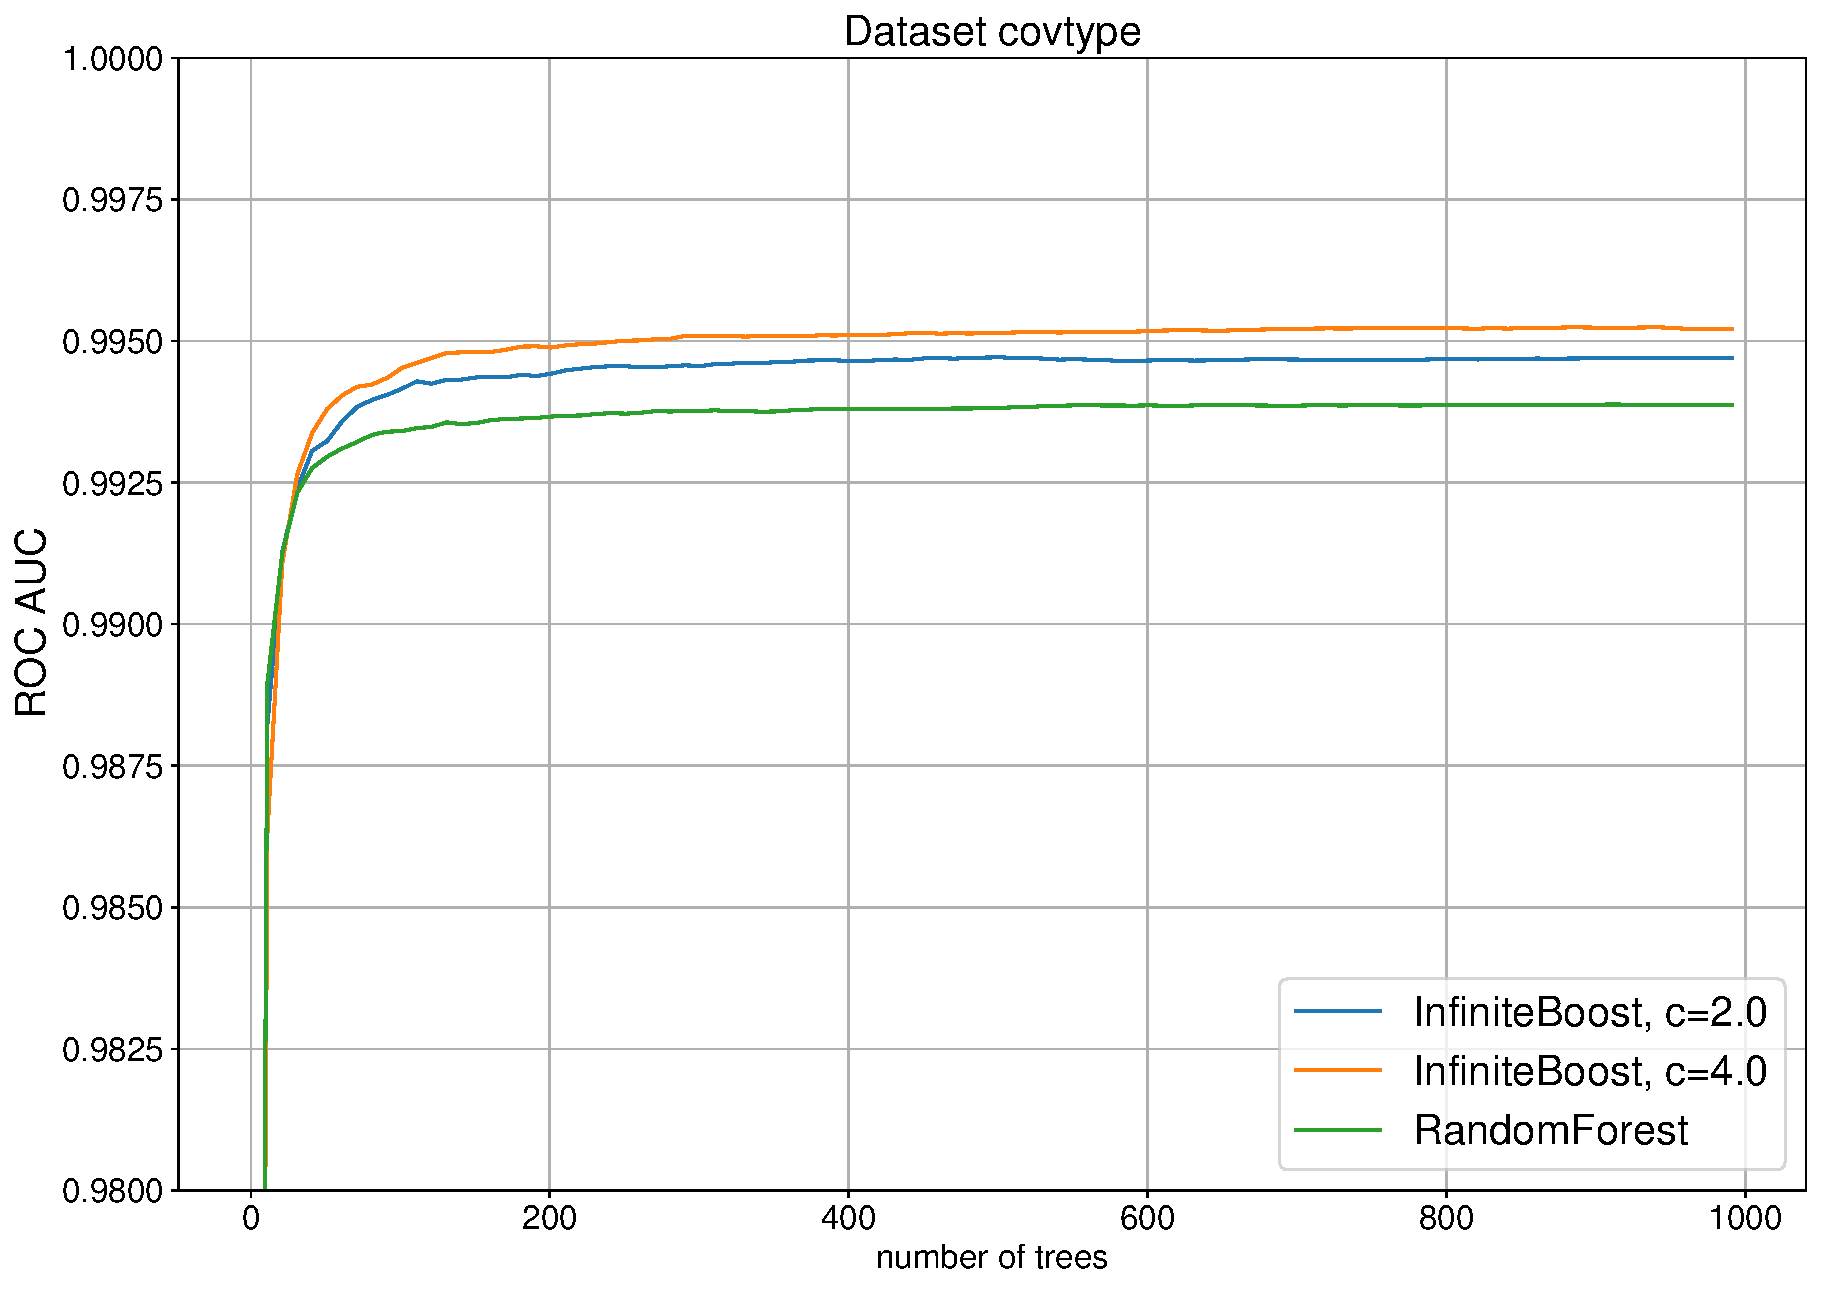
\includegraphics[width=1\linewidth]{../research/plots/forest_longrun_covtype.pdf}
      
      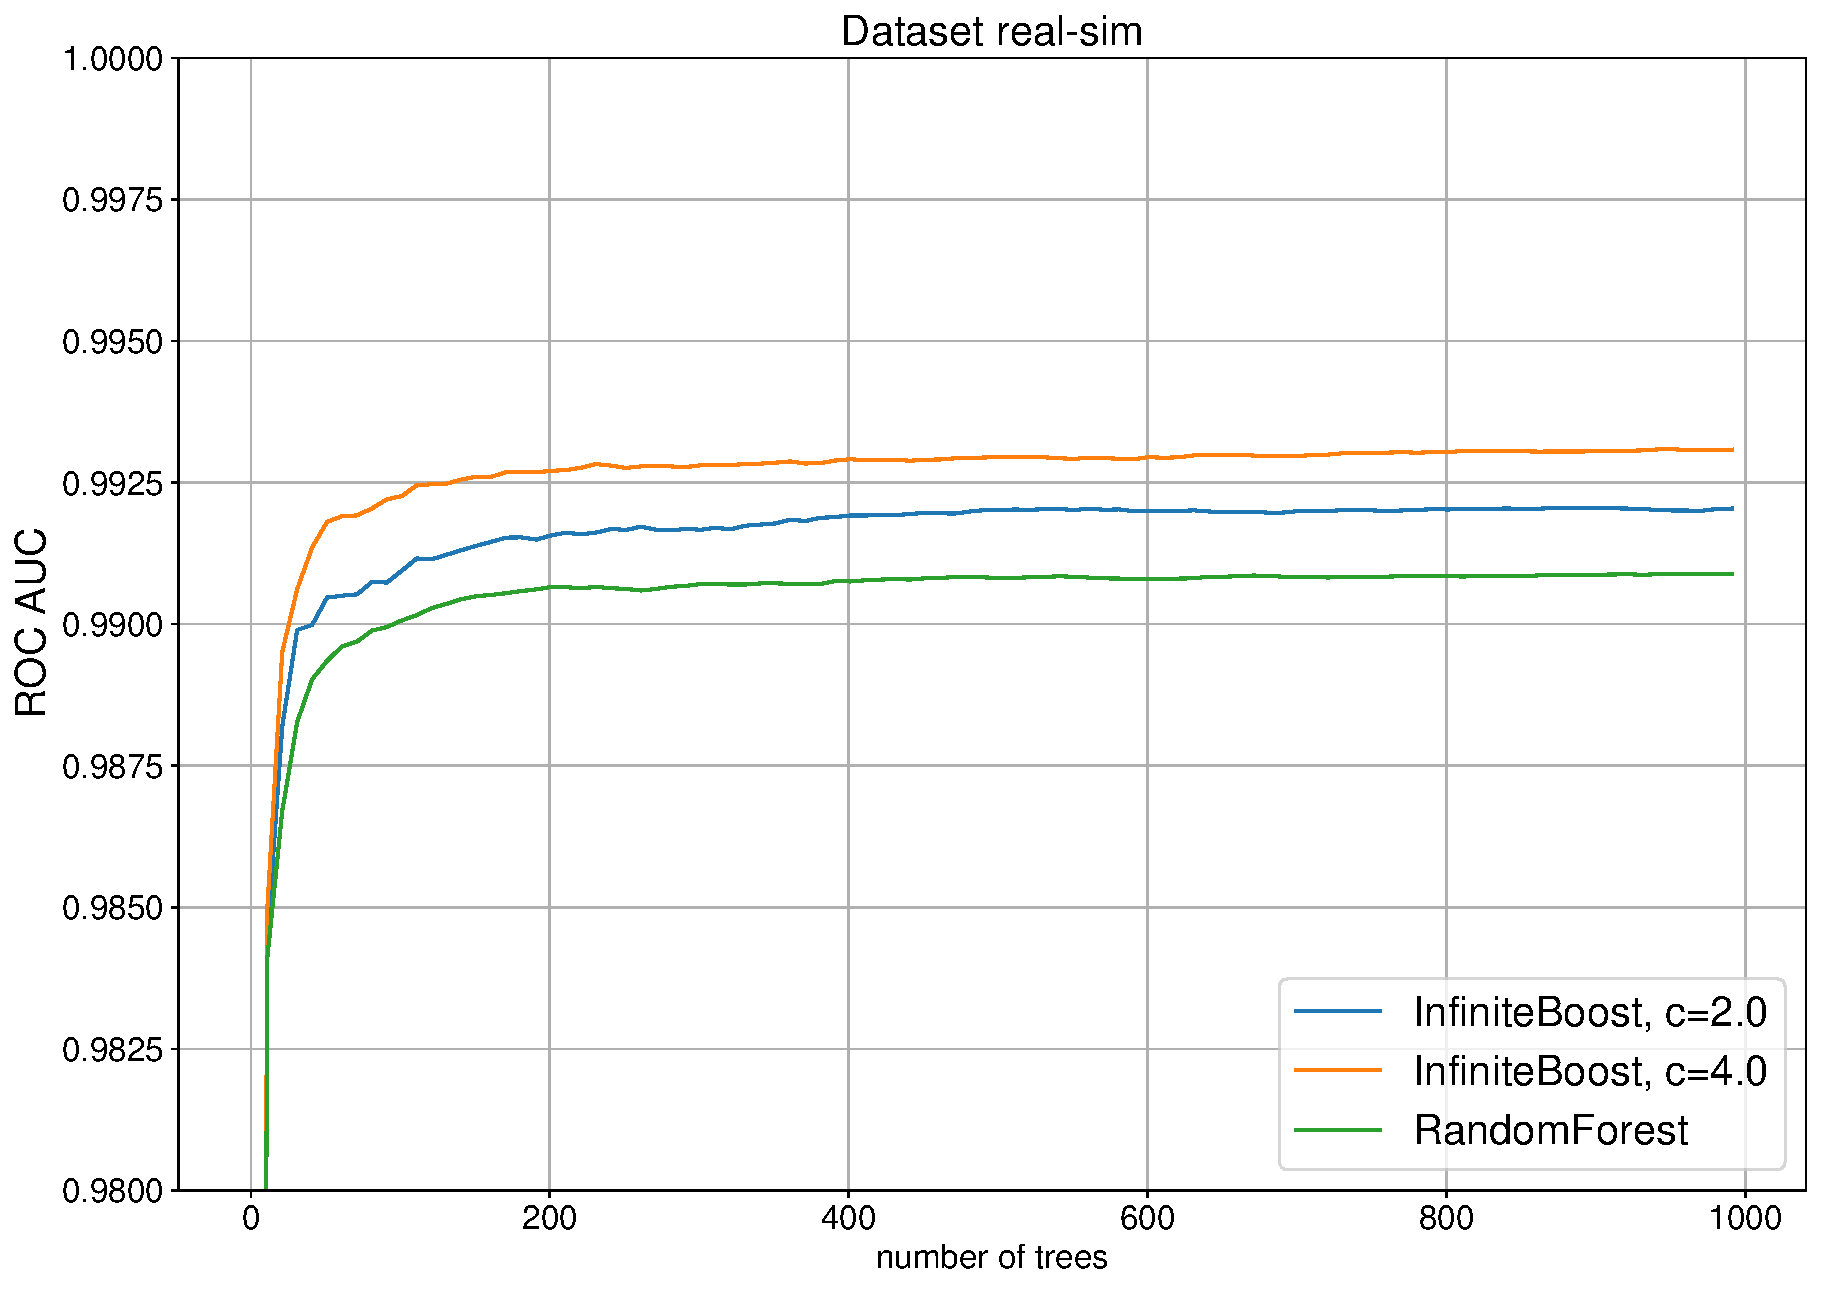
\includegraphics[width=1\linewidth]{../research/plots/forest_longrun_real-sim.pdf}
    \end{multicols}
    \caption{ROC AUC quality on covertype (left) and real-sim (right) datasets for random forest and infinite boosting with capacities $c=2$ and $c=4$. \label{fig:inf}}
  \end{figure*}
\else
  \begin{figure*}[!h]
    \centering
      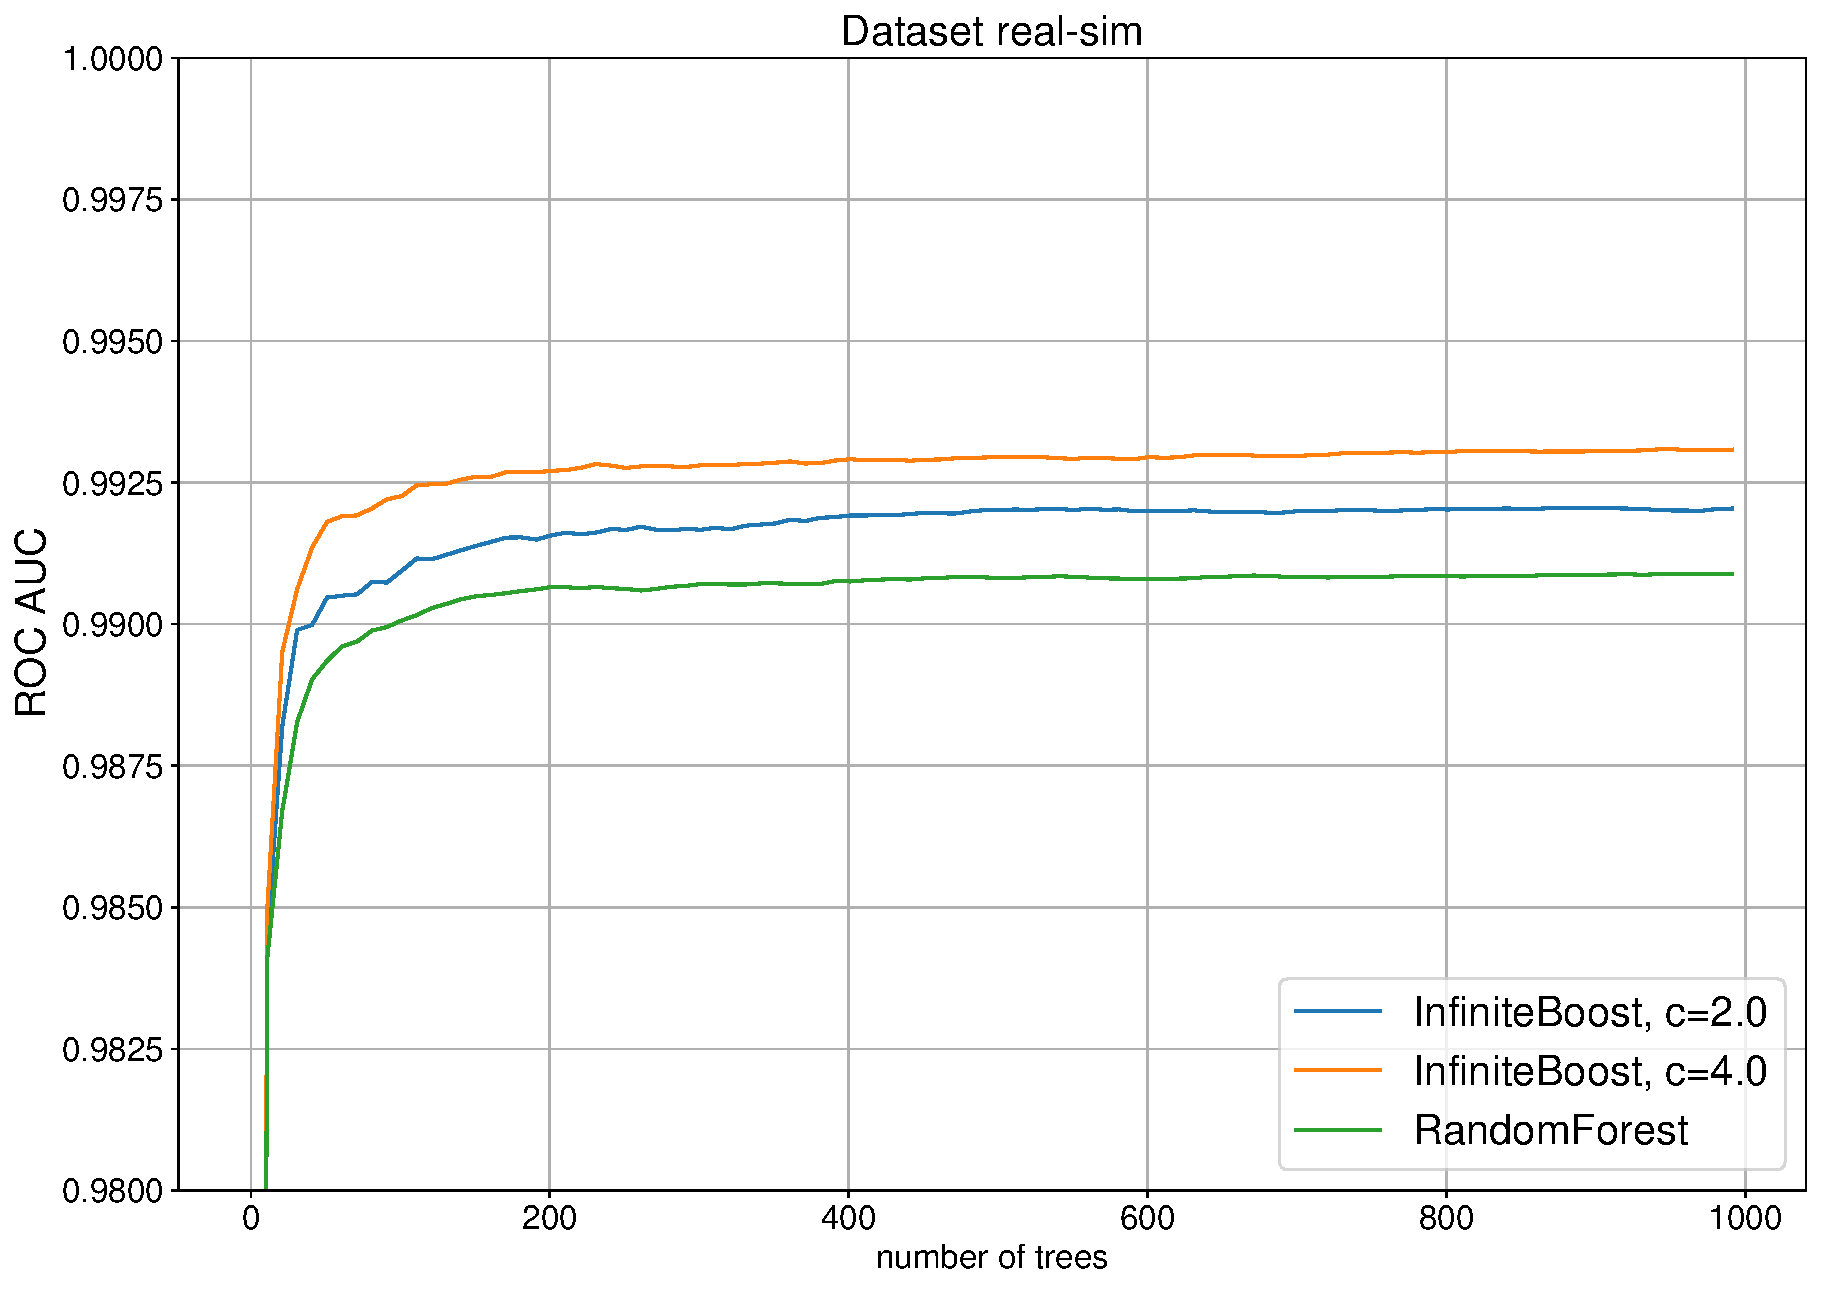
\includegraphics[width=0.5\linewidth]{../research/plots/forest_longrun_real-sim.pdf}
      \caption{ROC AUC quality on real-sim dataset for random forest and infinite boosting with capacities $c=2$ and $c=4$. \label{fig:inf}}
  \end{figure*}
\fi
